\newpage
\section{Ocaml Basics: Syntax, Types, and Semantics}

\subsection*{Strong Typing}

OCaml is a strongly typed language, meaning that operations between incompatible types are not allowed. Additionally, the underscore (\texttt{\_}) is used as a throwaway variable for values that are not intended to be used.

\begin{lstlisting}[language=OCaml, caption={Example of Strong Typing}]
    let x : int = 2
    let y : string = "two"
    let _ = x + y (* THIS IS NOT POSSIBLE *)
\end{lstlisting}

\noindent
This will result in the following error:
\begin{lstlisting}[language=Bash, caption={Error Message}]
    3 | let _ = x + y (* THIS IS NOT POSSIBLE *)
        ^ 
    Error: This expression has type string but an expression was expected of type int
\end{lstlisting}

\noindent
Demonstrating that, in OCaml, unlike other languages, operator overloading and implicit type conversions are not allowed.
This means, no adding strings and integers, floats and integers, etc. There are separate operators for each type.\\

\noindent
\textbf{Basic Ocaml Operators:}\\
Operators in OCaml behave just like other languages, with a few exceptions. Here are the basic operators at a quick
glance:

\vspace{.5em}
\begin{table}[h!]
    \centering
    \resizebox{\textwidth}{!}{%
    \begin{tabular}{|c|c|c|}
    \hline
    \rowcolor{OliveGreen!10}\textbf{Type}   & \textbf{Literals Examples}             & \textbf{Operators}           \\ \hline
    \texttt{int}    & \texttt{0, -2, 13, -023}      & \texttt{\textcolor{Wine}{+}, \textcolor{Wine}{-}, \textcolor{Wine}{*}, \textcolor{Wine}{/}, \textcolor{Wine}{mod}}      \\ \hline
    \texttt{float}  & \texttt{3., -1.01}            & \texttt{\textcolor{Wine}{+.}, \textcolor{Wine}{-.}, \textcolor{Wine}{*.}, \textcolor{Wine}{/.}}       \\ \hline
    \texttt{bool}   & \texttt{true, false}          & \texttt{\textcolor{Wine}{\&\&}, \textcolor{Wine}{||}, \textcolor{Wine}{not}}        \\ \hline
    \texttt{char}   & \texttt{'b', 'c'}             &                               \\ \hline
    \texttt{string} & \texttt{"word", "@*\&\#"}     & \textcolor{Wine}{$^\wedge$}                  \\ \hline
    \end{tabular}%
    }
    \caption{Basic OCaml Types, Literals, and Operators}
    \label{tab:ocaml-types}
\end{table}

\newpage 

\noindent
For emphasis:
\begin{Def}[OCaml Operators]

    \noindent
    \textbf{Operator Distinctions:}\\
    Operators for \snippet{int} and \snippet{float} are \textit{different}. For example:
    \begin{itemize}
        \item \snippet{+} (integer addition)
        \item \snippet{+.} (float addition)
        \item \snippet{$^\wedge$} (string concatenation)
    \end{itemize}
    
    \noindent
    Moreover, the \snippet{mod} operator is used for integer division. This is to 
    say that there is no implicit type conversion in OCaml.\\
    \rule{\textwidth}{0.4pt}

    \vspace{.3em}
    \noindent
    \textbf{No Operator Overloading:}\\
    OCaml has \underline{\textbf{no operator overloading}}, meaning operators are strictly tied to specific types.

    \vspace{.3em}
    \noindent
    \rule{\textwidth}{0.4pt}

    \vspace{.3em}
    \noindent
    \textbf{Comparison Operators:}\\
    Comparison operators are standard and can be used to compare expressions of the same type:
    \begin{itemize}
        \item \snippet{<}, \snippet{<=}, \snippet{>}, \snippet{>=}
    \end{itemize}

    \vspace{-.3em}
    \noindent
    \rule{\textwidth}{0.4pt}
    
    \noindent
    \textbf{Equality and Inequality:}

    \vspace{-.5em}
    \begin{itemize}
        \item Equality check: \snippet{=}
        \item Inequality check: is \snippet{<>} \textbf{and not}, \snippet{!=}
    \end{itemize}

    \vspace{-1em}
    
\end{Def}

\vspace{-1em}
\noindent
\begin{Def}[OCaml (in) Keyword]
    
Consider the expression below:
\begin{lstlisting}[language=OCaml, numbers=none]
    let x = 2 in x + x 
\end{lstlisting}

\noindent
The \snippet{in} keyword is used to bind the value of \snippet{x} to the expression \snippet{x + x}. This is a common pattern in OCaml.
In a sense we are saying, `` let $x$ stand for 2 in the expression $x + x$.''\\

This is similar to the prerequisite definition of the substitution operation (\ref{def:substitution}). Mathematically, we can think of this as:
\[
    [2/x](x + x) = 2 + 2
\]

\noindent
Where the value of 2 is substituted for $x$ in the expression $x + x$.

\end{Def}
\newpage 

\noindent
To illustrate this, Observe the diagram below:\\

\vspace{-1em}

\begin{figure}[h]
    {
    \setlength{\fboxsep}{10pt}
    \centering
    \fbox{\hspace{2em}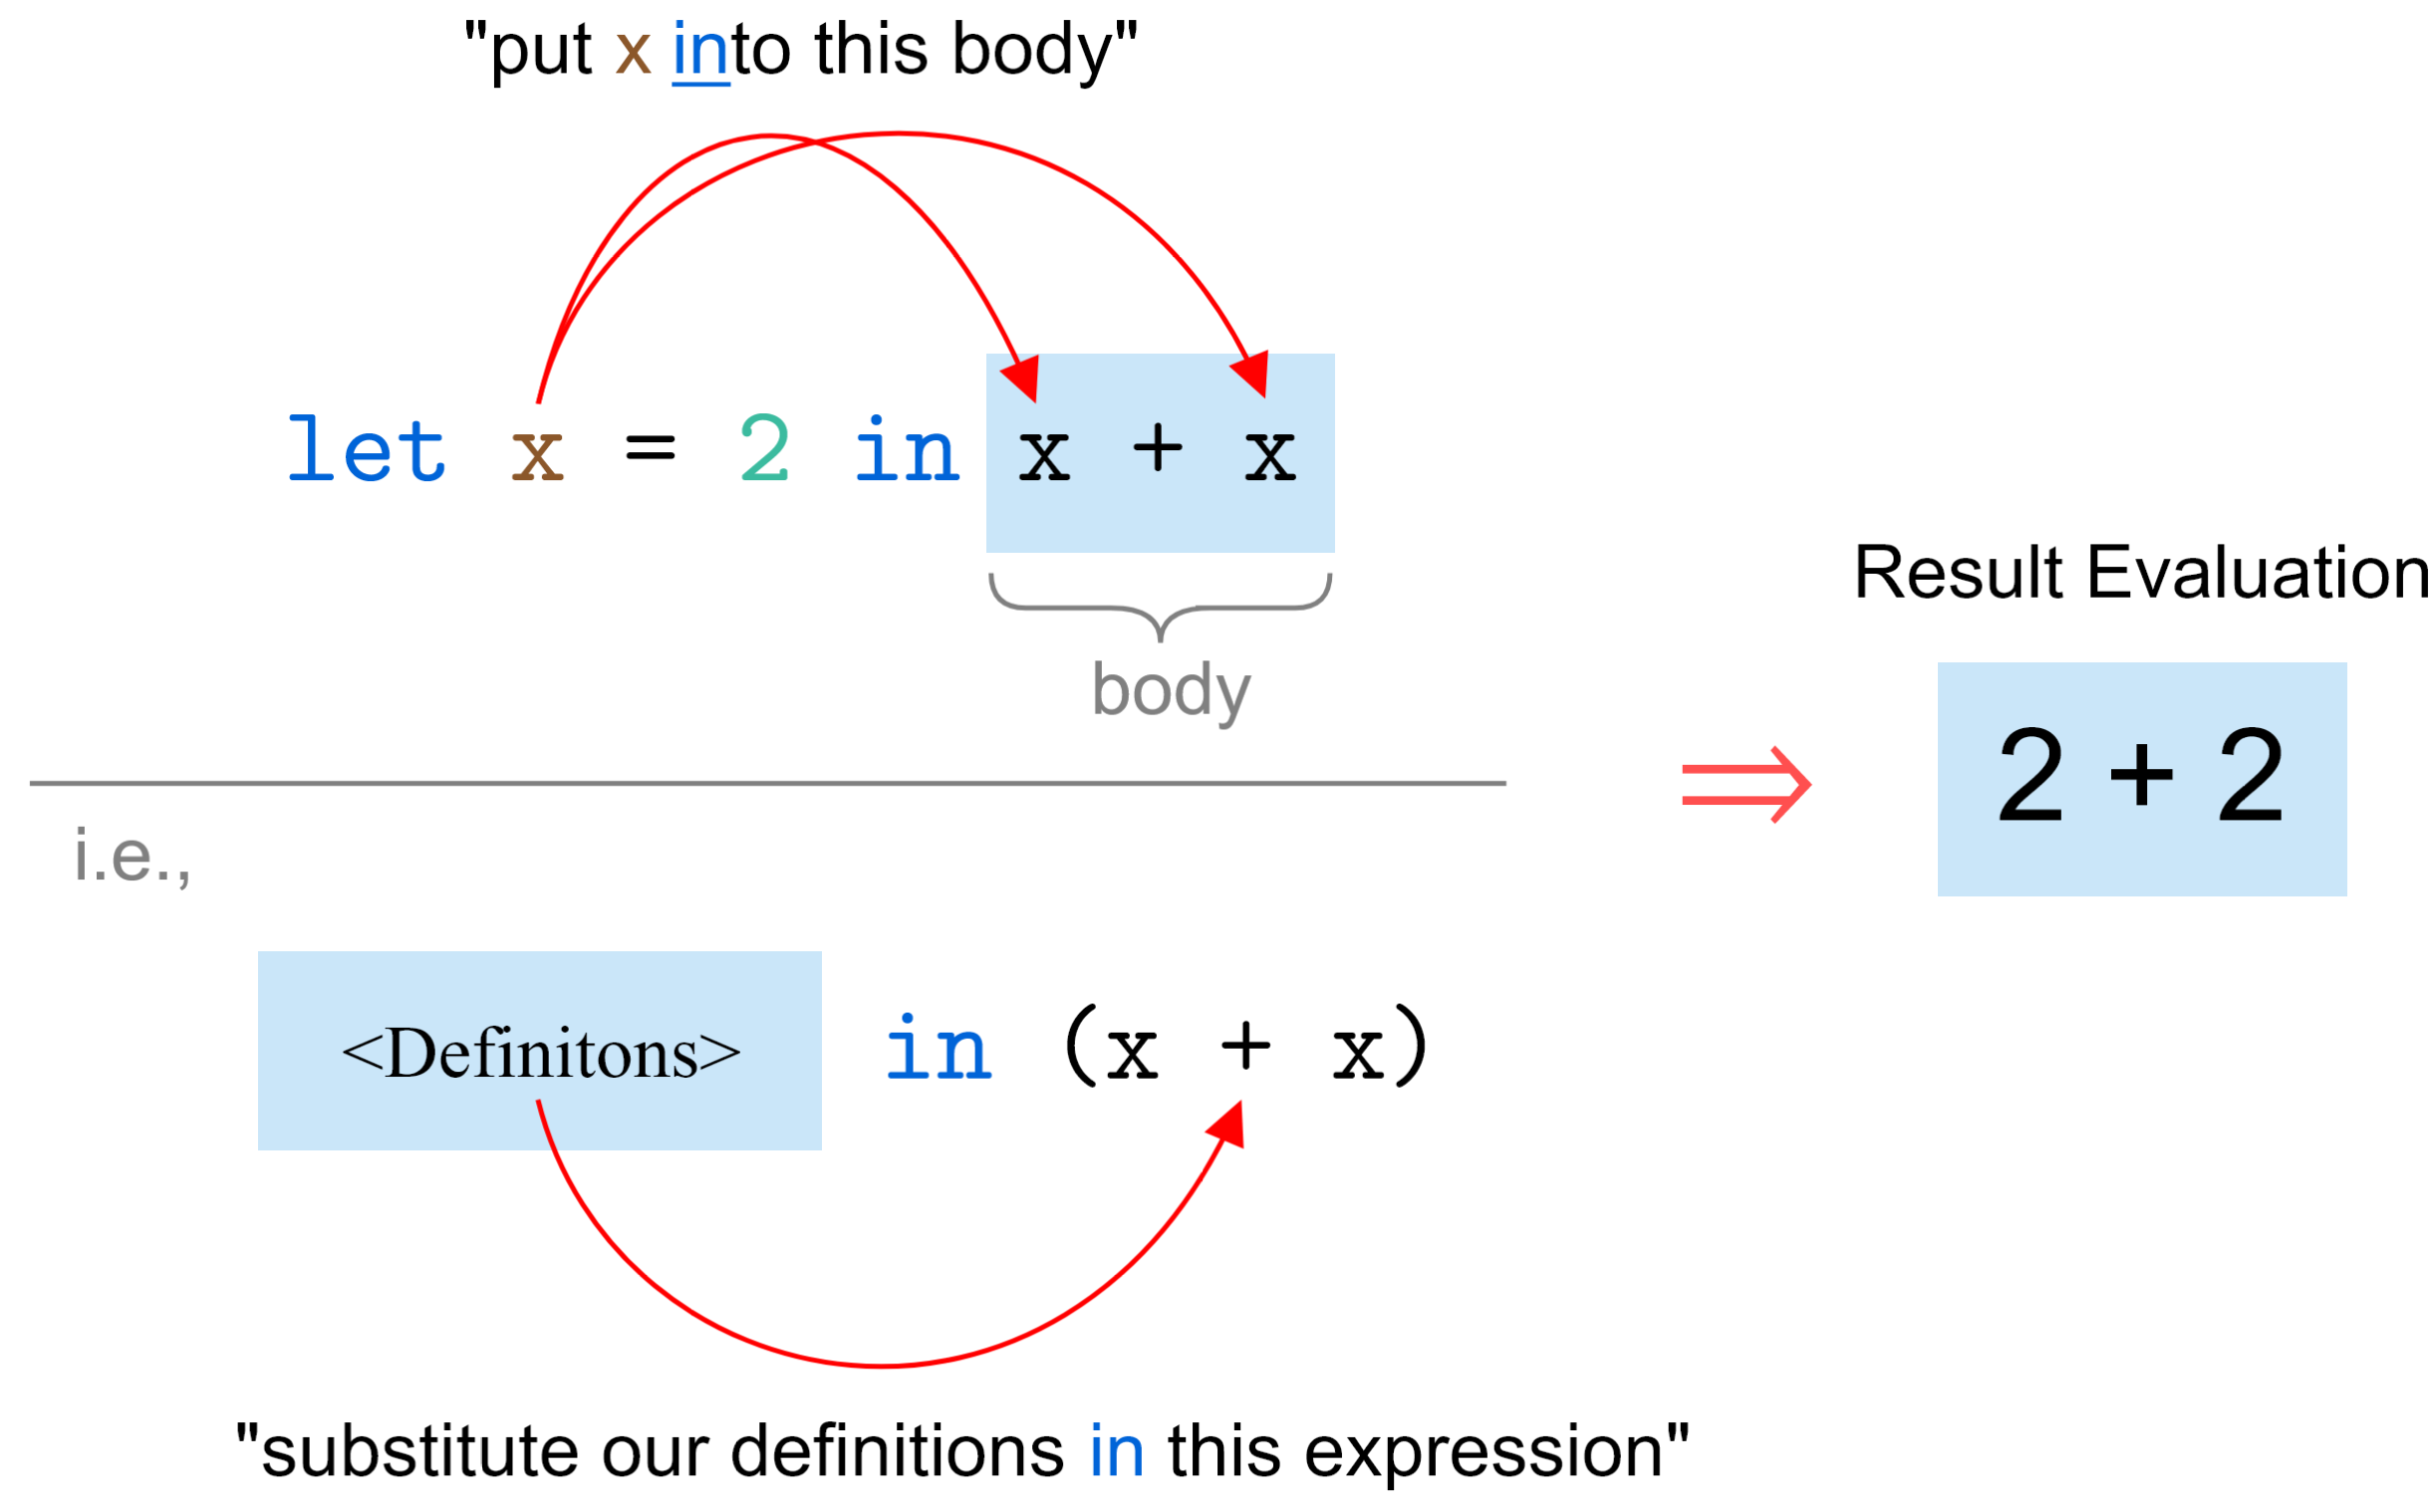
\includegraphics[width=0.8\textwidth]{Sections/Func/ocam/indef.png}\hspace{3em}}
    }
    \caption{The \snippet{in} Keyword in OCaml}
    
    \label{fig:ocaml-in}
\end{figure}



\vspace{-1em}
\noindent
To disect the roles of \textbf{syntax}, \textbf{semantics}, and \textbf{types} in the expression \snippet{let x = 2 in x + x}:

\begin{figure}[h]
    {
        \setlength{\fboxsep}{10pt}
    \centering
    \fbox{\hspace{4em} 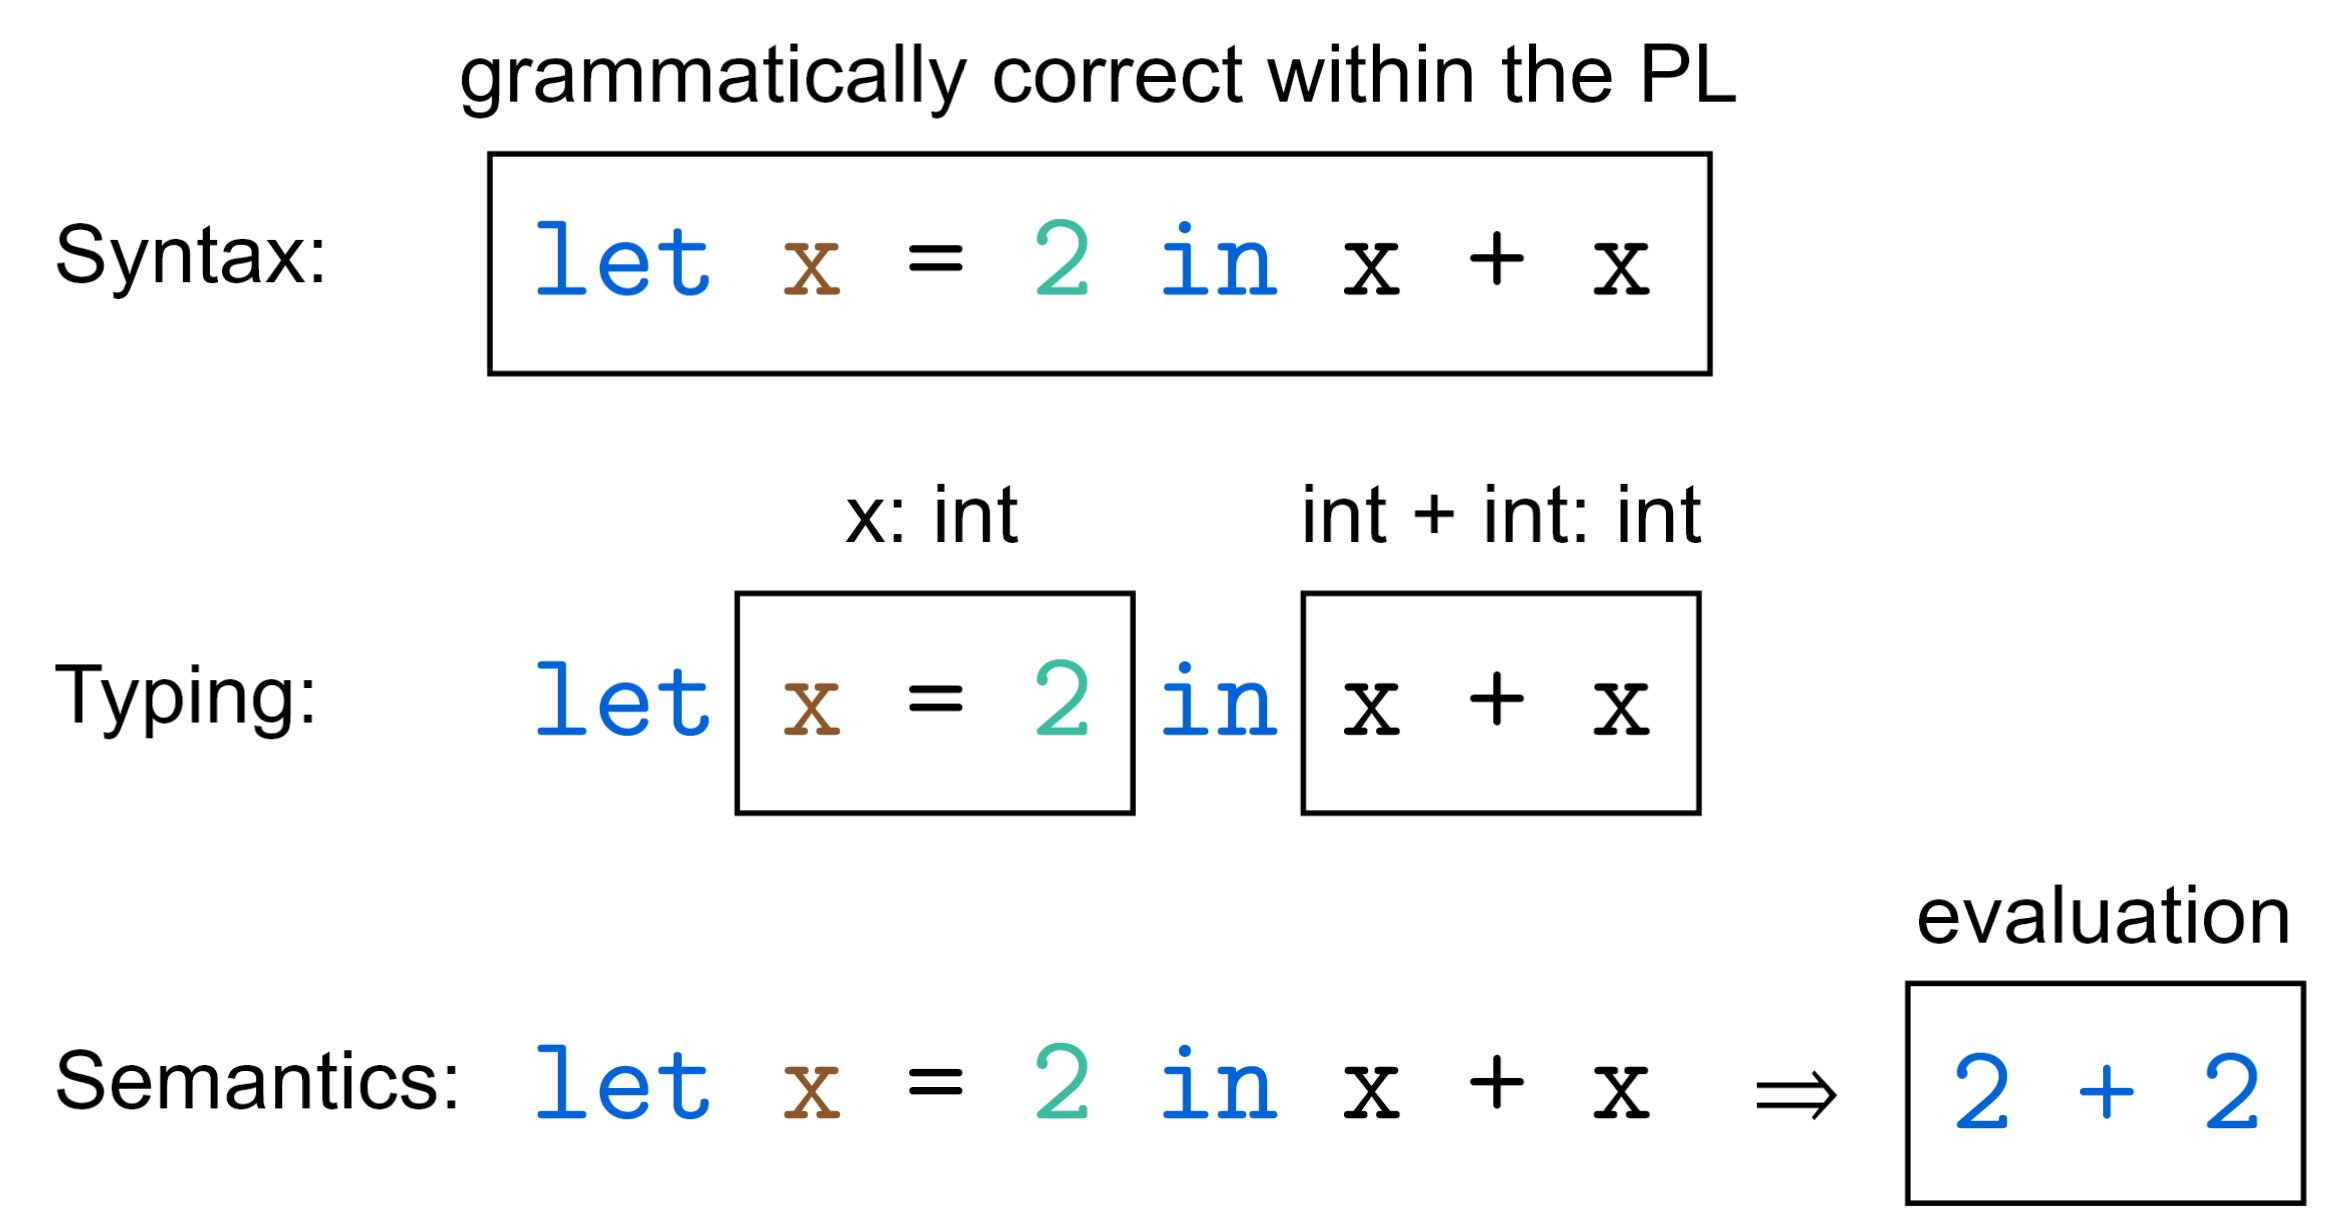
\includegraphics[width=.7\textwidth]{Sections/Func/ocam/sst.png}\hspace{5em}}
    }
    \caption{Syntax, Semantics, and Types in OCaml}
    \label{fig:ocaml-in2}
\end{figure}

\vspace{-1em}
\noindent
\begin{itemize}
    \item \textbf{Syntax}: The expression \snippet{let x = 2 in x + x} is a valid OCaml expression.
    \item \textbf{Typing}: Well-typed, as $x$ is an \snippet{int} and $x + x$ is an \snippet{int}.
    \item \textbf{Semantics}: After substitution, the expression evaluates to $2 + 2$.
\end{itemize}

\newpage 

\begin{Def}[Whitespace Agnostic]
    OCaml is \textbf{whitespace agnostic}, meaning that the interpreter does not rely on the presence or absence of whitespace to determine the structure of the code. Whitespace can be used freely for readability without affecting the semantics of the program. For example, the following expressions are equivalent:
    \begin{lstlisting}[language=OCaml, numbers=none, caption={Whitespace Agnostic Example}]
    let x = 1 + 2
    \end{lstlisting}

    and

    \begin{lstlisting}[language=OCaml, numbers=none]
    let x 
    = 1
      +
      2
    \end{lstlisting}

    \noindent
    Both produce the same result, as whitespace does not alter the meaning of the expression.
\end{Def}

\subsection{Understanding Functions in OCaml}
\label{subsec:func-ocaml}
In OCaml, functions do not require parentheses, arguments directly follow the function name. 
For example:
\begin{lstlisting}[language=OCaml]
    let add x y z = x + y + z in 
    let result = add 3 5 5
    (* semantically evaluates to 3 + 5 + 5 *)
\end{lstlisting}

\noindent
Here, the \snippet{add} function takes three arguments, \snippet{x}, \snippet{y}, and \snippet{z} which is substituted into \snippet{result} with arguments 3, 5, and 5.\\

\begin{Def}[Anonymous Functions]

An \textbf{anonymous function} is a one-time-use function that is not bound to a name. In OCaml, anonymous functions are created using the \snippet{fun} keyword.
They are useful for passing functions as arguments to other functions or for defining functions locally. For example:

\begin{lstlisting}[language=OCaml, numbers=none]
    let add x y z = x + y z
\end{lstlisting}
\noindent is equivalent to:
\begin{lstlisting}[language=OCaml, numbers=none]
    let add = fun x -> fun y -> fun z -> x + y + z
\end{lstlisting}

\noindent
These are formally known as \textbf{lambda expressions}, where in \textbf{lambda calculus} \snippet{fun x -> e} is written 
as ``$\lambda x.e$'', s.t., $\lambda$ denotes the anonymous function, $x$ the argument, and $e$ the expression.
The add function is equivalent to, $\lambda x.\lambda y.\lambda z.x + y + z$, in lambda calculus.

\end{Def}

\newpage

\noindent
Functions with multiple arguments can be thought of as nested anonymous functions, where variables are passed 
down the chain of functions. To illustrate:

\begin{figure}[h]
    {
    \setlength{\fboxsep}{16pt}
    \centering
    \fbox{\hspace{2em}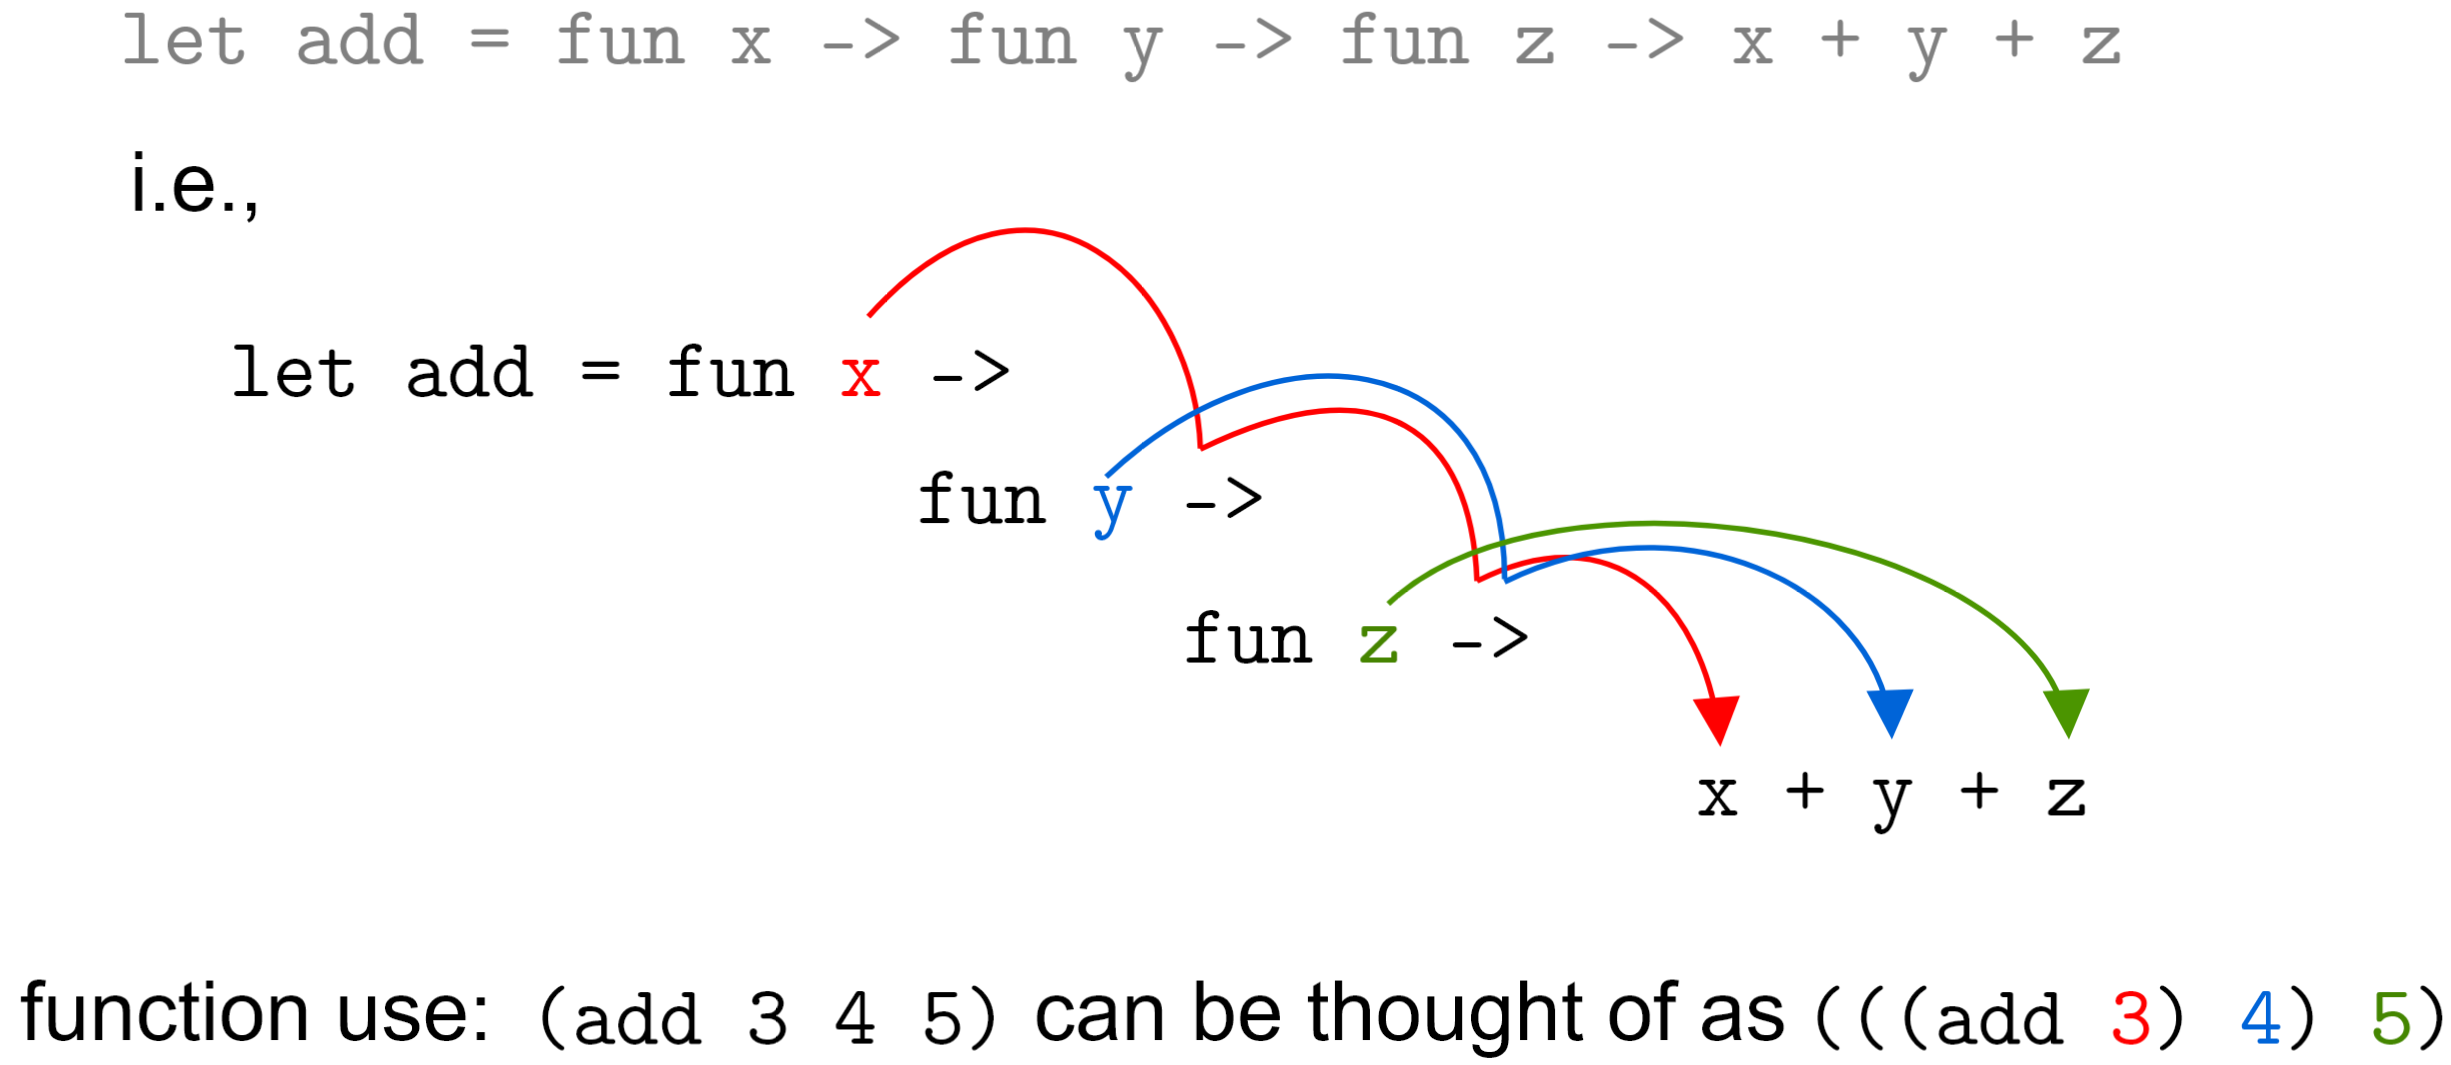
\includegraphics[width=0.8\textwidth]{Sections/Func/ocam/curry.png}\hspace{3em}}
    }
    \caption{Anonymous Functions in OCaml}
    
    \label{fig:ocaml-anon}
\end{figure}

\vspace{-1em}
\noindent
Alternatively, we may illustrate an analogous example with scoped functions in a pseudo syntax:

\begin{figure}[h]
    {
    \setlength{\fboxsep}{0pt}
    \centering
    \fbox{\hspace{8.7em}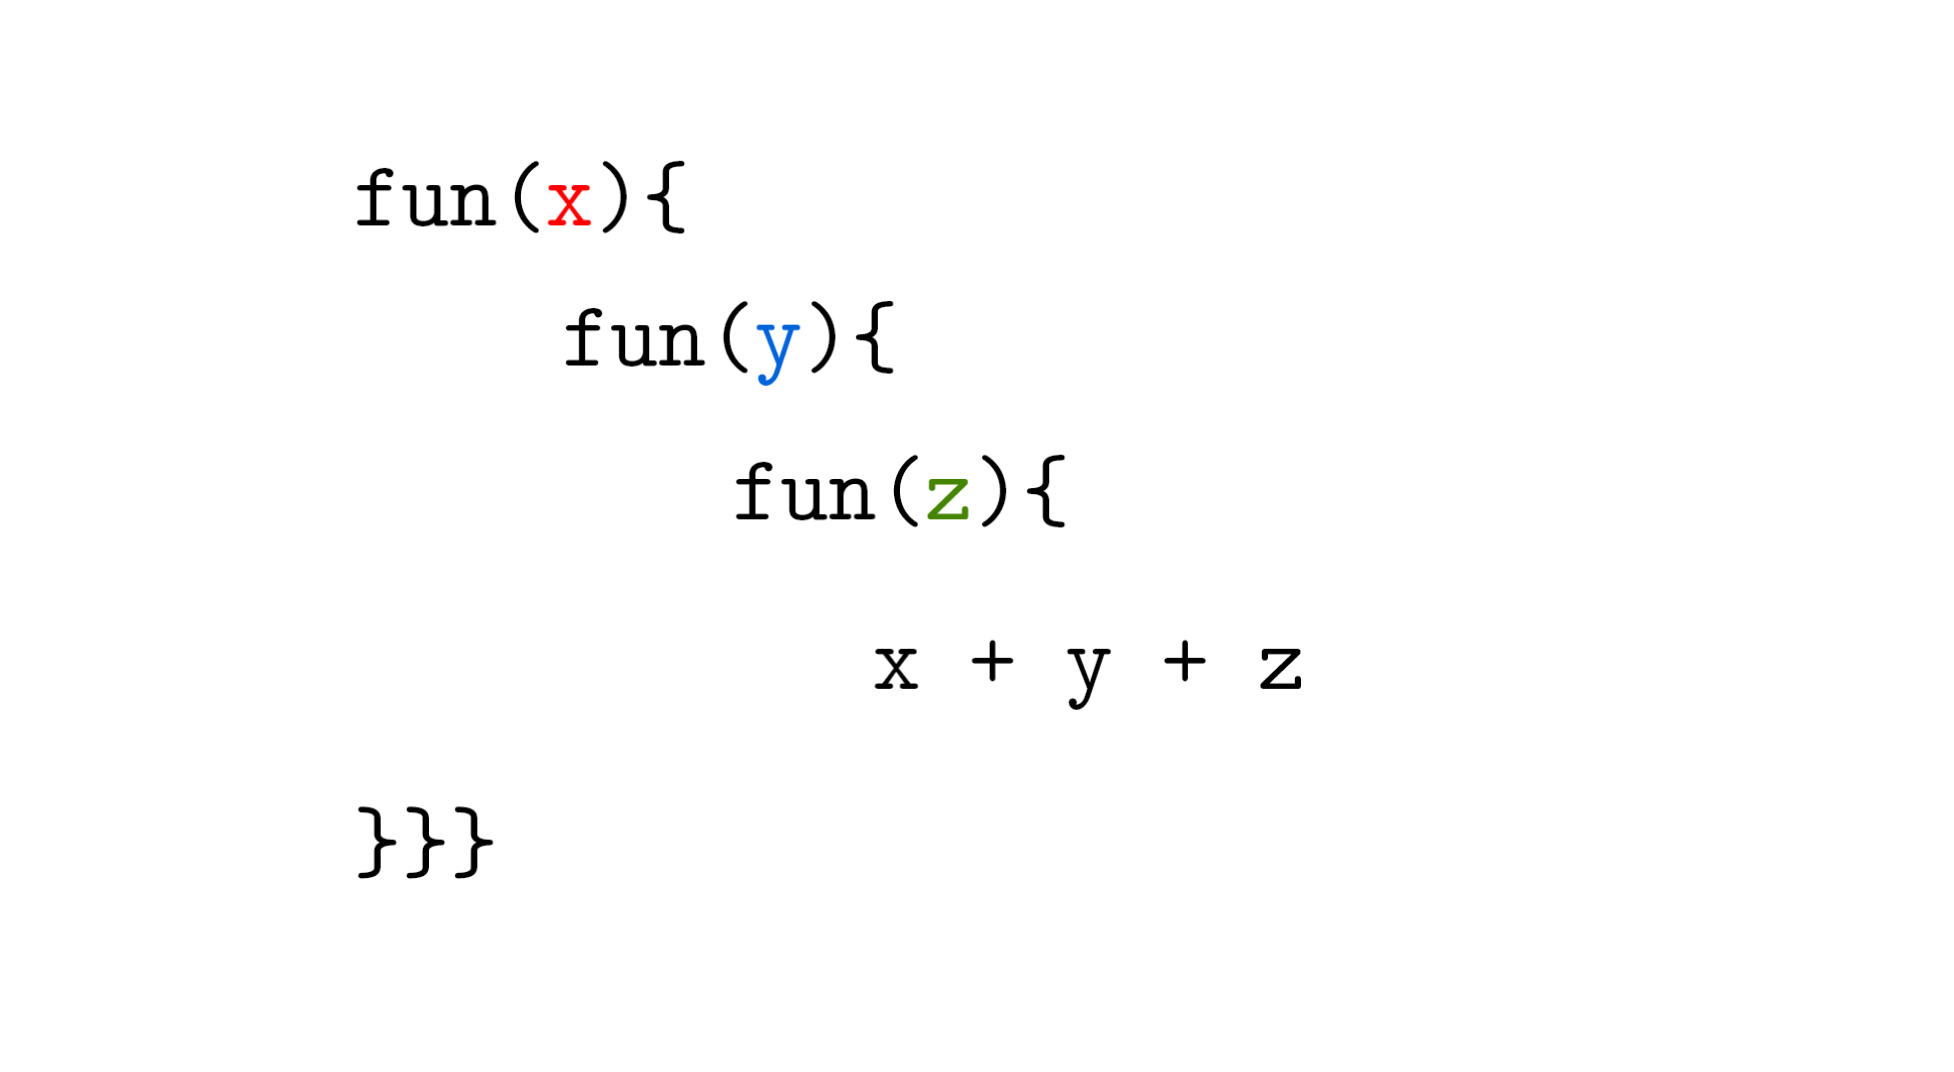
\includegraphics[width=0.6\textwidth]{Sections/Func/ocam/curry2.png}\hspace{8em}}
    }
    \caption{Nested Functions Pseudo-code Example}
    
    \label{fig:ocaml-anon2}
\end{figure}

\vspace{-.5em}
\noindent
Where $x$ is a local variable of the outer-most function within scope of the inner functions, and so on with $y$ and $z$.
This is the concept known as \textbf{currying}.

\begin{Tip}
    Lambda calculus was developed by \textbf{Alonzo Church} in the 1930s at Princeton University. Church was the doctoral advisor of \textbf{Alan Turing}, the creator of the Turing Machine (1936), a theoretical model that laid the groundwork for modern computation.
    
    Curry functions were introduced by \textbf{Haskell Curry} around the 1940-1950s as he worked in the U.S. He expanded upon combinatory logic, emphasizing breaking down functions into a sequence of single-argument functions.
\end{Tip}
    

\newpage

\begin{Def}[Curried Functions]

A \textbf{curried function} is a function that, when applied to some arguments, returns another function that takes the remaining arguments. For example:
\[
\texttt{add x y = x + y}
\]
is internally equivalent to:
\[
\texttt{add = fun x -> (fun y -> x + y)}
\]

In OCaml, functions are \textbf{curried} by default. This means that a function of multiple arguments is treated as a sequence of single-argument functions.
\end{Def}

\vspace{1em}
\noindent
We let \snippet{add} stand for \snippet{fun x -> fun y -> x + y}. Therefore in reality we are doing:
\begin{lstlisting}[language=OCaml]
    (fun x -> fun y -> x + y) 3 5
\end{lstlisting}

\noindent
This is know as \textbf{Application}, as we are \textit{applying} arguments to a function.

\vspace{1em}
\begin{Def}[Application]

    \textbf{Application} is the process of applying arguments to a function. \textbf{Full application} is when all 
    arguments are applied to a function. For example:

    \begin{lstlisting}[language=OCaml, numbers=none]
        (fun x -> fun y -> x + y) 3 5
    \end{lstlisting}

    \noindent
    Here, the function \snippet{fun x -> fun y -> x + y} is fully applied to the arguments 3 and 5.\\

    \noindent
    \textbf{Partial application} is when only some arguments are applied to a function, which evaluates to another function 
    accepting the remaining arguments. For example:

    \begin{lstlisting}[language=OCaml, numbers=none]
        (fun x -> fun y -> x + y) 3
    \end{lstlisting}

    \noindent
    Here, the function \snippet{fun x -> fun y -> x + y} is partially applied to the argument 3, resulting in a new function
    \snippet{fun y -> 3 + y}.\\

    \noindent
    \textbf{In Lambda Calculus} we may represent this as:
    \begin{align*}
        (\lambda x. \lambda y. (x + y))&\ 3\ 5 \rightarrow\\
        (\lambda y. (3 + y))&\ 5 \rightarrow\\
        (3 + 5) \hspace{.4em} &
    \end{align*}
    In this process, arguments are sequentially applied to the corresponding variables.
\end{Def}

\newpage 


\begin{Def}[Side Effects in OCaml]

    A \textbf{side effect} refers to any change in the state of the program or its environment caused by a function or expression. 
    This includes modifying variables, printing to the console, writing to a file, or interacting with external systems:
    
    \begin{lstlisting}[language=OCaml, caption={Function Without a Side Effect}, numbers=none]
    let square x = x * x
    (* This function computes the square of a number.
       It has no side effects as it doesn't change 
       state or interact with the outside world. *)
    \end{lstlisting}
    
    \begin{lstlisting}[language=OCaml, caption={Function With a Side Effect}, numbers=none]
    let print_square x =
      let result = x * x in
      Printf.printf "The square of %d is %d\n" x result
    (* This function prints the square of a number.
       It has a side effect: printing to the console. *)
    \end{lstlisting}
    \end{Def}
    

\begin{Def}[The (unit) Type in OCaml]

The \snippet{unit} type represents a value that carries no information. It is denoted by \snippet{()}, which is both the type and the sole value of \snippet{unit}. Functions returning \snippet{unit} are typically used for side effects.

\begin{lstlisting}[language=OCaml, caption={Unit Type and Value}, numbers=none]
    let x = ()
    (* x has the type unit and the value (). *)
\end{lstlisting}

\begin{lstlisting}[language=OCaml, caption={Function Returning Unit}, numbers=none]
    let print_hello () = print_endline "Hello"
    (* This function takes unit as an argument and returns unit. *)
\end{lstlisting}

The \snippet{unit} type ensures that functions used for their effects are explicit in their intent, making it clear they do not return meaningful data.
\end{Def}

\newpage

\begin{Def}[Void Functions in OCaml]

\label{def:void}
\textbf{Void functions} are functions that perform actions but do not return meaningful values. 
These functions take \snippet{unit} as an argument and return \snippet{unit}, making their purpose explicit.

\begin{lstlisting}[language=OCaml, caption={Void Function Example}, numbers=none]
    let log_message () = print_endline "Logging message" 
    in log_message ()
    (*Evaluates to "Logging message", which takes and returns a unit.*)
\end{lstlisting}

\noindent
Void functions are often seen in the main entry point of an OCaml program:
\begin{lstlisting}[language=OCaml, caption={Using \snippet{let ()} in the Main Function}, numbers=none]
    let () =
    print_endline "Program starting...";
    (* Additional program logic here. *)
\end{lstlisting}
\end{Def}

\begin{Def}[Skeleton Code]
    
    To write skeleton code one can use the \snippet{assert} keyword, though of course running this function will result in an error.

    \begin{lstlisting}[language=OCaml, caption={Skeleton Code Example}, numbers=none]
        let skeleton () = assert false
        (* This function is a placeholder for unwritten code. *)
    \end{lstlisting}

\noindent
\end{Def}

\begin{Def}[Multiple Function Arguments]

    Applying expressions without parentheses may lead to unexpected results. For example:

    \begin{lstlisting}[language=OCaml, caption={Incorrect Function Application}, numbers=none]
        (fun x y -> x + y) 3 5 * 2
        (* Evaluates: 16 as ((fun x y -> x + y) 3 5) * 2 *)
    \end{lstlisting}
    \noindent
    As it takes the immediate arguments that are available, to avoid this, use parentheses to group expressions correctly:
    \begin{lstlisting}[language=OCaml, caption={Correct Function Application}, numbers=none]
        (fun x y -> x + y) 3 (5 * 2)
        (* Evaluates: 13 *)
    \end{lstlisting}
\end{Def}

\newpage
\subsection{If-Expressions}
In OCaml, \textbf{if-expressions} are used to conditionally evaluate expressions. This behaves similarly to other PLs with a few distinctions.

\begin{Def}[Ocaml if-then-else]

    In OCaml, \textbf{if-statements} follow the form: \snippet{if <condition> then <expr1> else <expr2>}, i.e., 
    if the condition is true, then \snippet{expr1} is evaluated, else \snippet{expr2} is evaluated:
    \begin{lstlisting}[language=OCaml, caption={If-Expression: Divisible by 2}, numbers=none]
        fun x -> if x mod 2 = 0 then "even" else "odd"
    \end{lstlisting}

    \noindent
    Here, the anonymous function finds if $x$ is divisible by 2, evaluating to \snippet{"even"} if true, or otherwise \snippet{"odd"}.

    \noindent
    \rule{\textwidth}{0.4pt}

    \vspace{.3em}
    \noindent
    \textbf{Typing}: The \snippet{then} and \snippet{else} expressions must evaluate to the same type. 
    So the following expression is \textbf{invalid}:

    \begin{lstlisting}[language=OCaml, caption={Invalid If-Expression}, numbers=none]
        fun x -> if x mod 2 = 0 then "even" else 0 (* INVALID *)
    \end{lstlisting}

    \noindent
    \rule{\textwidth}{0.4pt}

    \vspace{.3em}
    \noindent
    \textbf{Else If}: In OCaml, there is no \snippet{else if} keyword. Instead, nested if-expressions are used to achieve the same effect.

    \begin{lstlisting}[language=OCaml, caption={Else If Example}, numbers=none]
        fun x -> 
            if x mod 3 = 0 then 
                "divisible by 3"
            else if x mod 5 = 0 then
                "divisible by 5" 
            else "not divisible by 2 or 3"
    \end{lstlisting}
\end{Def}
\begin{Def}[Conditional Assignment]

    A \textbf{conditional assignment} is a variable is assignment based off a condition:
    \begin{lstlisting}[language=OCaml, caption={Conditional Assignment}, numbers=none]
        fun x -> let result = if x mod 2 = 0 then "even" else "odd" 
        in result
        (* Evaluates result as "even" or "odd" depending on x *)
    \end{lstlisting}
\end{Def}


\newpage 


\subsection{Type Hinting in OCaml}
\noindent
Type hinting is a way to explicitly specify the types of variables or function parameters in OCaml. This can be useful for documentation, readability, and debugging purposes.\\

\begin{Def}[Type Hinting in OCaml]

    In OCaml, \textbf{type hinting} allows programmers to explicitly specify the types of variables or function parameters. While type hints are not necessary due to OCaml's strong and static type system, 
    they can help clarify intent and make code easier to understand, especially for larger projects.\\

   
    \begin{lstlisting}[language=OCaml, caption={Adding Type Annotations to Functions}, numbers=none]
    let add (x : int) (y : int) : int = x + y
    (* Explicitly states that x and y are integers, which results as an integer. *)
    \end{lstlisting}
    \noindent
   
    \begin{lstlisting}[language=OCaml, caption={Adding Type Annotations to Variables}, numbers=none]
    let name : string = "OCaml"
    (* Explicitly states that name is a string. *)
    \end{lstlisting}


    \begin{lstlisting}[language=OCaml, caption={Type Hinting in Anonymous Functions}, numbers=none]
    (fun (x : float) (y : float) -> x *. y) 3.0 4.2;;
    (* Multiplies two floats stating explicitly typing arguments as floats. *)
    \end{lstlisting}

    Though possibly adding redundancy, theoretically we may type any expression in OCaml.
\begin{lstlisting}[language=OCaml, caption={Type Hinting in Conditional Expressions}, numbers=none]
    ((fun (x : int) -> 
            if x mod 2 = 0 then "even" 
            else "odd"
     ) : int -> string) 5 
    (* Evaluates to "odd" *)
\end{lstlisting}
\end{Def}

\newpage

\subsection{OCaml Data Structures: Arrays, Lists, and Tuples}

There are arrays, lists, and tuples in OCaml. While OCaml is not a purely functional language, we will treat it as such in this text.

\begin{Def}[Lists in OCaml]

    A \textbf{list} in OCaml is an ordered, immutable collection of elements of the same type, 
    created via square brackets \snippet{[ ]} semicolon separated:
    \begin{lstlisting}[language=OCaml, caption={Defining a List}, numbers=none]
    [1; 2; 3; 4]
    (*Syntax: [e1;e2;e3;...;en] *)

    [[1; 2]; [3; 4]; [5; 6]]
    (* 2D list of type: int list list *)   
    \end{lstlisting}

    \begin{lstlisting}[language=OCaml, caption={Indexing a List \& Finding Length}, numbers=none]
    List.nth [1; 2; 3; 4] 2
    (*Evaluates to 3; Syntax: List.nth <list> <index> *)
    
    List.length [1; 2; 3; 4]
    (*Evaluates to 4; Syntax: List.length <list> *)
    \end{lstlisting}

    \begin{lstlisting}[language=OCaml, caption={Joining Lists}, numbers=none]
    [1; 2] @ [3; 4]
    (*Evaluates to [1; 2; 3; 4]; 
      Syntax: <list1> @ <list2> *)

    1 :: [2; 3; 4]
    (* ``::'' is the cons operator;
      Evaluates to [1; 2; 3; 4]; Syntax: <element> :: <list>
      Equiv. to: 1 :: 2 :: 3 :: 4 :: [] I.e., 1 :: (2 :: (3 :: (4 :: [])))
    *)
    \end{lstlisting}
    \begin{lstlisting}[language=OCaml, caption={Pattern Matching on Lists}, numbers=none]
    let rec sum_list l =
        match l with
        | [] -> 0
        | x :: xs -> x + sum_list xs
    in 
    sum_list [1; 2; 3; 4]
    (* Evaluates to 10 as 1 + 2 + 3 + 4 *)
    \end{lstlisting}
\end{Def}

\newpage

\vfill

\begin{Def}[Arrays in OCaml]

    \textbf{Arrays} are a fixed-length random access (indexable) mutable collection of elements with the same type.
    They are created with brackets and vertical bars \snippet{[| |]}:
    \begin{lstlisting}[language=OCaml, caption={Defining and Modifying an Array}, numbers=none]
    [|1; 2; 3; 4|]
    (* Creates an array of integers: [|1; 2; 3; 4|] *)
    \end{lstlisting}

    \begin{lstlisting}[language=OCaml, caption={2D Array}, numbers=none]
    [|[|1; 2|]; [|3; 4|]|]
    (* Creates a 2D array of type: int array array *)    
    \end{lstlisting}

    \begin{lstlisting}[language=OCaml, caption={Arrays.make: Prefill Length Array}, numbers=none]
    Array.make 3 0
    (*Evaluates to [|0; 0; 0|]; 
      Syntax: Array.make <length> <initial_value> *)
    \end{lstlisting}

    \begin{lstlisting}[language=OCaml, caption={Accessing Array Elements}, numbers=none]
    let arr = [|1; 2; 3; 4|] in arr.(2)
    (*Evaluates to 3; 
      Syntax: <array>.(<index>) *)
    \end{lstlisting}

    \begin{lstlisting}[language=OCaml, caption={Arrays.init: Creating Array with Function}, numbers=none]
    Array.init 5 (fun i -> i * 2)
    (*Evaluates to [|0; 2; 4; 6; 8|] where i is the index; 
      Syntax: Array.init <length> <function> *)
    \end{lstlisting}

    \begin{lstlisting}[language=OCaml, caption={Mutating Array Elements}, numbers=none]
    let arr = [|1; 2; 3; 4|] in arr.(2) <- 5
    (*Evaluates [|1; 2; 5; 4|]; 
      Syntax: <array>.(<index>) <- <new_value> *)
    \end{lstlisting}

    \begin{lstlisting}[language=OCaml, caption={Length of Array}, numbers=none]
    Array.length [|1; 2; 3; 4|]
    (*Evaluates to 4; 
      Syntax: Array.length <array> *)
    \end{lstlisting}
\end{Def}

\vfill

\newpage


\begin{Def}[Tuples in OCaml]

    A \textbf{tuple} in OCaml is an ordered collection of elements, where each element can have a different type. Tuples are immutable and their size is fixed. They are created using parentheses with elements separated by commas:
    \begin{lstlisting}[language=OCaml, caption={Defining a Tuple}, numbers=none]
    (3, 4)
    (*Syntax: (e1, e2, ..., en) *)
    \end{lstlisting}

    \begin{lstlisting}[language=OCaml, caption={2D Tuple}, numbers=none]
    ((1, 2), (3, 4))
    (* 
    2D tuple of type: (int * int) * (int * int) 
    *)
    \end{lstlisting}

    \begin{lstlisting}[language=OCaml, caption={Mixed Type Tuple}, numbers=none]
    (3, "hello", true, 4.2)
    (*
    Mixed type tuple (3, "hello", true, 4.2): int * string * bool * float 
    *)
    \end{lstlisting}

    \begin{lstlisting}[language=OCaml, caption={Accessing Tuple via Pattern Matching}, numbers=none]
    match (3, 4) with (x, y) -> x + y
    (*Evaluates to 7; 
      Syntax: match <tuple> with (<pattern>) -> <expr> *)
    \end{lstlisting}
    \noindent
    More on \snippet{match} (Pattern Matching) in the next section.

    \begin{lstlisting}[language=OCaml, caption={Accessing Tuple via Decomposition}, numbers=none]
    let (x, y) = (3, 4)
    (*Evaluates to x = 3, y = 4; 
      Syntax: let (<pattern>) = <tuple> *)
    \end{lstlisting}

    \noindent
    \textbf{Note:} There is no built-in functions to index or retrieve a length of a tuple in OCaml. Tuples 
    are seen as a single entity, where pattern matching is typically utilized to access elements.
\end{Def}

\newpage 
\subsection{Pattern Matching \& Switch-Case Absence}

In OCaml, \underline{\textbf{There is no switch-case statement}}, pattern matching is used instead:

\begin{Def}[OCaml Pattern Matching (match ... with ...)]

    \textbf{Pattern matching} in OCaml is a mechanism for inspecting and deconstructing data based on its structure. 
    The \snippet{match ... with} expression evaluates a value and compares it against a series of patterns, executing the first matching case. Its syntax is as follows:
    
    \begin{lstlisting}[language=OCaml, caption={Pattern Matching Syntax}, numbers=none]
    match <expression> with
    | <pattern1> -> <result1>
    | <pattern2> -> <result2>
    | ...
    | <patternN> -> <resultN>
    \end{lstlisting}
    
    \noindent
    Here, \snippet{<expression>} is the value being evaluated, and each \snippet{<pattern>} represents a condition or structure to match.
    
    \begin{lstlisting}[language=OCaml, caption={Matching an Integer}, numbers=none]
    fun x ->
      match x with
      | 0 -> "zero"
      | 1 -> "one"
      | 2 | 3 -> "two or three"
      | _ -> "other";;
    
    describe_number 0;; (* Evaluates to "zero" *)
    describe_number 5;; (* Evaluates to "other" *)
    \end{lstlisting}

    \begin{lstlisting}[language=OCaml, caption={Matching Multiple Arguments}, numbers=none]
    fun x y ->
      match (x, y) with
      | (0, 0) -> "origin"
      | (0, _) -> "x-axis"
      | (_, 0) -> "y-axis"
      | _ -> "other"
    (* Utilizing a tuple to match multiple arguments *)
    \end{lstlisting}
    
    \begin{itemize}
        \item \textbf{Underscore (\_):} A wildcard pattern that matches anything not explicitly listed.
        \item \textbf{Multiple Patterns:} Separate patterns with \snippet{|} to match multiple cases.
        \item \textbf{Deconstruction:} Use pattern matching to extract values from compound data structures such as tuples, lists, or variants.
    \end{itemize}
\end{Def}

\newpage 
    
\subsection{Looping: Recursion, Tail-End Recursion}

In functional programming, looping is typically achieved through \textbf{recursion}. Unlike imperative programming, where loops rely on mutable state, 
recursion allows us to iterate by repeatedly calling a function while unravelling our expressions. While OCaml is not a purely functional language and does provide \snippet{for} and \snippet{while} loops, 
in the context of this text, we will only use recursion for looping.

\vspace{2em}
\begin{Def}[Ocaml Recursion]

Recursion is the process of a function calling itself. Any and all recursive functions need the keyword
\snippet{rec} to be used in OCaml:

\noindent

\begin{lstlisting}[language=OCaml, caption={Summing to $n$ Using Recursion}, numbers=none]
    let rec sum_to_n n =
        if n = 0 then 0
        else n + sum_to_n (n - 1)
    in 
    sum_to_n 5
    (* Evaluates to 15 as 5 + 4 + 3 + 2 + 1 + 0 *)
\end{lstlisting}

\begin{lstlisting}[language=OCaml, caption={Fibonacci Sequence Using Recursion}, numbers=none]
    let rec fibonacci n =
        if n <= 1 then n
        else fibonacci (n - 1) + fibonacci (n - 2)
    in 
    fibonacci 6
    (* Evaluates to 8 as 0, 1, 1, 2, 3, 5, 8 *)
    
\end{lstlisting}

\begin{lstlisting}[language=OCaml, caption={Sum an Array of Integers Using Recursion}, numbers=none]
    let rec sum_arr arr i =
        if i <= 0 then 0
        else arr.(i - 1) + sum_arr arr (i - 1)
    in
    let my_array = [|1; 2; 3; 4; 5|] in
    sum_arr my_array (Array.length my_array)
    (* Evaluates to 15 as 1 + 2 + 3 + 4 + 5 *)
\end{lstlisting}

\end{Def}

\newpage

\begin{Def}[Tail-End Recursion]

    Tail-end recursion refers to a type of recursion where the recursive call is the \emph{last operation} performed in the function. 
    This allows the OCaml compiler to reuse the same stack frame through \textbf{tail call optimization (TCO)}, helping avoid stack overflow errors.
    
    \begin{lstlisting}[language=OCaml, caption={Non-Tail-Recursive Factorial Function}, numbers=none]
    let rec factorial n =
        if n <= 1 then 1
        else n * factorial (n - 1)
    (* The multiplication (n * ...) occurs after the recursive call. *)
    \end{lstlisting}
    
    \noindent The above function \textbf{is not tail-recursive} as for \snippet{n} to be multiplied by the result of\\
    \snippet{factorial (n - 1)}. The recursive call must be evaluated first to get an answer, forcing us to track of intermediate stacks possibly leading to a stack overflow.
    Instead, we can pass an accumulated result as an argument to the function known as the \textbf{accumulator}:
    
    \begin{lstlisting}[language=OCaml, caption={Tail-Recursive Factorial Function}, numbers=none]
    let rec factorial n acc =
        if n <= 1 then acc
        else factorial (n - 1) (n * acc)
    (* The recursive call is the last operation performed. *)
    \end{lstlisting}

    \noindent To use the above we can call \snippet{... in factorial n 1} to start the recursion with an initial accumulator of 1.
    To abstract this, we can define a auxiliary helper function to hide the accumulator from the user:

    \begin{lstlisting}[language=OCaml, caption={Tail-Recursive Factorial Function with Helper}, numbers=none]
    let factorial n =
        let rec aux n acc =
            if n <= 1 then acc
            else aux (n - 1) (n * acc)
        in aux n 1
    in factorial 5
    (* Evaluates to 120 as 5! = 5 * 4 * 3 * 2 * 1 *)
    \end{lstlisting}

    \begin{lstlisting}[language=OCaml, caption={Tail-Recursive Summation of Positive Even Numbers}, numbers=none]
    let rec sum_even n acc =
        if n <= 0 then acc
        else if n mod 2 = 0 then sum_even (n - 1) (acc + n)
        else sum_even (n - 1) acc
    in sum_even 5 0
    (* Evaluates to 6 as 4 + 2 + 0 = 6. *)
    (* Despite two recursive calls they are independent of each other. *)
    \end{lstlisting}
        
\end{Def}

\newpage

\subsection{Strings, Characters, and Printing in OCaml}

Strings, characters, and printing behave much the same as in other languages, with some unique functions and syntax in OCaml.

\begin{Def}[Strings in OCaml]

Strings in OCaml are immutable and allow for various operations, such as concatenation, slicing, and transformation:

    \begin{lstlisting}[language=OCaml, caption={Creating and Concatenating Strings}, numbers=none]
    let greeting = "Hello" ^ " " ^ "World!"
    (* Evaluates to "Hello World!"; 
    Syntax: <string1> ^ <string2> *)
    \end{lstlisting}

    \begin{lstlisting}[language=OCaml, caption={Getting the Length of a String}, numbers=none]
    String.length "Hello"
    (* Evaluates to 5; 
    Syntax: String.length <string> *)
    \end{lstlisting}

    \begin{lstlisting}[language=OCaml, caption={Accessing a Character in a String}, numbers=none]
    "Hello".[1]
    (* Evaluates to 'e'; 
    Syntax: <string>.[<index>] *)
    \end{lstlisting}

    \begin{lstlisting}[language=OCaml, caption={Slicing a String}, numbers=none]
    String.sub "Hello World" 6 3
    (* Evaluates to "Wor"; 
    Syntax: String.sub <string> <start> <length> *)
    \end{lstlisting}


    \begin{lstlisting}[language=OCaml, caption={Converting to Uppercase}, numbers=none]
    String.uppercase_ascii "hello"
    (* Evaluates to "HELLO"; 
    Syntax: String.uppercase_ascii <string> *)
    \end{lstlisting}

    \begin{lstlisting}[language=OCaml, caption={String Equality}, numbers=none]
    "hello" = "world" (* Evaluates to false*)
    "hello" = "hello" (* Evaluates to true*)
    \end{lstlisting}
\end{Def}

\newpage 

\begin{Def}[Characters in OCaml]

    Characters in OCaml are individual elements of strings and are represented using single quotes (e.g., `a'). 
    Unlike strings, characters are immutable single units that cannot be directly concatenated or manipulated as strings:
    
    \begin{lstlisting}[language=OCaml, caption={Defining Characters}, numbers=none]
    let char_a = 'a'
    (* A character is represented with single quotes. *)
    \end{lstlisting}
    
    \begin{lstlisting}[language=OCaml, caption={Comparing Characters}, numbers=none]
    'a' < 'b'
    (* Evaluates to true; 
       Syntax: <char1> < <char2> *)
    \end{lstlisting}
    
    \begin{lstlisting}[language=OCaml, caption={Converting Characters to Strings}, numbers=none]
    Char.escaped 'a'
    (* Evaluates to "a"; 
       Syntax: Char.escaped <char> *)
    \end{lstlisting}
    
    \begin{lstlisting}[language=OCaml, caption={Converting Characters to Integers}, numbers=none]
    Char.code 'a'
    (* Evaluates to 97 (ASCII code of 'a'); 
       Syntax: Char.code <char> *)
    \end{lstlisting}
    
    \begin{lstlisting}[language=OCaml, caption={Converting Integers to Characters}, numbers=none]
    Char.chr 97
    (* Evaluates to 'a' (ASCII character for 97); 
       Syntax: Char.chr <int> *)
    \end{lstlisting}
    
    \begin{lstlisting}[language=OCaml, caption={Checking if a Character is Uppercase}, numbers=none]
    Char.uppercase_ascii 'a'
    (* Evaluates to 'A'; 
       Syntax: Char.uppercase_ascii <char> *)
    \end{lstlisting}
    
\end{Def}

\newpage
\begin{Def}[Printing in OCaml]

    Displays information on the terminal, typically for debugging or interacting with users:
    
    \begin{lstlisting}[language=OCaml, caption={Printing a String}, numbers=none]
    print_endline "Hello, World!"
    (* Prints "Hello, World!" followed by a newline;
       Syntax: print_endline <string> *)
    \end{lstlisting}
    
    \begin{lstlisting}[language=OCaml, caption={Printing Integers, Floats, and Characters}, numbers=none]
    print_int 42; print_newline ()
    (* Prints "42" followed by a newline;
       Syntax: print_int <int>; print_newline () *)
    
    print_float 3.14159; print_newline ()
    (* Prints "3.14159" followed by a newline;
        Syntax: print_float <float>; print_newline () *)

    print_char 'A'; print_newline ()
    (* Prints "A" followed by a newline;
        Syntax: print_char <char>; print_newline () *)
    \end{lstlisting}
    
    \textbf{Note:} If strictly using \snippet{stdlib320} then \snippet{Printf} is not available.
    \begin{lstlisting}[language=OCaml, caption={Formatted Printing with Printf}, numbers=none]
    Printf.printf "The number is: %d\n" 42
    (* Prints "The number is: 42" with formatted output;
       Syntax: Printf.printf <format> <value> *)
    \end{lstlisting}
    
    \begin{lstlisting}[language=OCaml, caption={Formatted Printing for Floats}, numbers=none]
    Printf.printf "Pi is approximately: %.2f\n" 3.14159
    (* Prints "Pi is approximately: 3.14" with 2 decimal places;
       Syntax: Printf.printf <format> <float> *)
    \end{lstlisting}
    
    \begin{lstlisting}[language=OCaml, caption={Printing Multiple Values}, numbers=none]
    Printf.printf "Name: %s, Age: %d\n" "Alice" 30
    (* Prints "Name: Alice, Age: 30" with formatted output;
       Syntax: Printf.printf <format> <value1> <value2> *)
    \end{lstlisting}

    
    \begin{lstlisting}[language=OCaml, caption={Using Printf.eprintf for Error Messages}, numbers=none]
    Printf.eprintf "Error: %s\n" "File not found"
    (* Prints "Error: File not found" to the standard error output. *)
    \end{lstlisting}
    
    \end{Def}

\newpage 

\subsection{Conversions in OCaml}

In OCaml implicit type conversions are not allowed, so we must explicitly convert between types when needed:

\begin{Def}[Common Conversions in OCaml]

\begin{lstlisting}[language=OCaml, caption={Integer and Float Conversions}, numbers=none]
float_of_int : int -> float

int_of_float : float -> int
\end{lstlisting}

\begin{lstlisting}[language=OCaml, caption={Character and Integer Conversions}, numbers=none]
int_of_char : char -> int

char_of_int : int -> char
\end{lstlisting}

\begin{lstlisting}[language=OCaml, caption={Boolean and String Conversions}, numbers=none]
string_of_bool : bool -> string

bool_of_string : string -> bool

bool_of_string_opt : string -> bool option
\end{lstlisting}

\begin{lstlisting}[language=OCaml, caption={String and Integer Conversions}, numbers=none]
string_of_int : int -> string

int_of_string : string -> int

int_of_string_opt : string -> int option
\end{lstlisting}

\begin{lstlisting}[language=OCaml, caption={String and Float Conversions}, numbers=none]
string_of_float : float -> string

float_of_string : string -> float

float_of_string_opt : string -> float option
\end{lstlisting}

\end{Def}

\newpage

\subsection{Defining Custom Types: Variants and Records}

In OCaml, we can define new types and structures to better organize our data and improve readability. This is especially useful when working with complex data structures. In particular, \textbf{records} provide a more user-friendly alternative to tuples by allowing named fields, while \textbf{variants} let us define custom types that can hold different kinds of values.

\vspace{2em}

\begin{Def}[Variants in OCaml]

A \textbf{variant} is a custom type that can take multiple forms. This is similar to an \textbf{enumeration} or a \textbf{sum type} in other languages. Variants are defined using the \snippet{type} keyword, followed by multiple constructors.

\begin{lstlisting}[language=OCaml, caption={Defining and Using Variants Correctly}, numbers=none]
(* Define a variant type for operating systems *)
    type os =
    | Windows
    | MacOS
    | Linux
    | BSD // <-- Constructor

    (* Function to describe the OS with explicit typing *)
    let describe_os (system : os) : string =
    match system with
    | Windows -> "A proprietary OS developed by Microsoft."
    | MacOS -> "A Unix-based OS developed by Apple."
    | Linux -> "An open-source OS based on the Linux kernel."
    | BSD -> "A Unix-like OS known for its security and stability."

    (* Correct Usage *)
    let my_os : os = Linux
    let description = describe_os my_os
    (* Evaluates to: "An open-source OS based on the Linux kernel." *)

    (* Incorrect Usage *)
    let unknown_os = Solaris
    (* Error: Unbound constructor Solaris *)
\end{lstlisting}
\end{Def}

\newpage

\begin{Def}[Records in OCaml]

A \textbf{record} is a immutable data structure that groups multiple values together. Each value is associated with a field name and accessors.

    \begin{lstlisting}[language=OCaml, caption={Defining and Using Records}, numbers=none]
    (* Define a record type for a person *)
    type person = {
    name : string;
    age : int;
    }

    (* Function to greet a person with explicit typing *)
    let greeting =
        let greet (p : person) : string =
            "Hello, " ^ p.name ^ "! You are " ^ string_of_int p.age ^ " years old."
        in
        let alice : person = { name = "Alice"; age = 30 } in
        greet alice
    (* Evaluates to: "Hello, Alice! You are 30 years old." *)
    \end{lstlisting}

\begin{lstlisting}[language=OCaml, caption={Incorrect Usage Example}, numbers=none]
...
    (* Attempting to create a record with a missing field *)
    let bob = { name = "Bob" }
    (* Error: Some record fields are undefined (age is missing). *)

    (* Using an incorrect type for a field *)
    let carol = { name = "Carol"; age = "twenty-five" }
    (* Error: This expression has type string but an expression was expected of type int. *)
\end{lstlisting}

    \begin{lstlisting}[language=OCaml, caption={Updating Records}, numbers=none]
    ...
    (fun name ->
        let alice = { name = "Alice"; age = 30 } in
        let _ = print_endline ("Original: " ^ alice.name) in
        let alice = { alice with name = name } in
        let _ = print_endline ("Updated: " ^ alice.name)
    ) "Bob"
    (* Prints:
    Original: Alice
    Updated: Bob
    *)
\end{lstlisting}
\end{Def}

\newpage 

% field punning

\begin{Def}[Variant (of) Keyword]

    We can define variant types to refer to a specific record type:

    \begin{lstlisting}[language=OCaml, caption={Variants Carrying Record Fields}, numbers=none]
    (* Defining a Record *)
    type sep_Rect = { base: float; height: float }

    (* Defining a Variant *)
    type shape = 
      | Circle of float
      | Rect of sep_Rect
      | Triangle of { sides: float * float; angle: float }
    (* Triangle is of record type with two fields: sides and angle *)

    (* Function to calculate the area of a shape *)
    let area (s : shape) =
        match s with
        | Rect r -> r.base *. r.height
        | Triangle { sides = (a, b) ; angle } -> Float.sin angle *. a *. b
        | Circle r -> r *. r *. Float.pi
    in 
    let my_shape : shape = Triangle { sides = (3.0, 4.0); angle = 2.0 }
    in area my_shape
    (* short handing ``angle=angle'' to ``angle'' (field punning) *)
    (* Evaluates to 10.9115691219081796 *)
    
    \end{lstlisting}
\end{Def}

\begin{Def}[Type Checking in OCaml]

    In OCaml, \textbf{type checking} is performed at \textbf{compile-time}, meaning we can't check types at runtime. Therefore we 
    must use variants and pattern matching to conditionally check types:

    \begin{lstlisting}[language=OCaml, caption={Using Variants for Type Checking}, numbers=none]
    type int_or_string =
        | Int of int
        | String of string

    let typeof t =
        match t with
        | Int x -> print_endline (string_of_int x ^ ": is Integer")
        | String x -> print_endline (x ^ ": is String")

    let _ = typeof (Int 42)    (* Output: 42: is Integer *)
    let _ = typeof (String "hi") (* Output: hi: is String *)
    \end{lstlisting}
\end{Def}


\newpage 

\subsection{Handling Absence of Values with Options}

In many programming languages, you might be familiar with the concept of a \textbf{null} value to represent the absence of a value. However, using \texttt{null} can lead to unexpected runtime errors if not handled carefully. OCaml avoids this pitfall by using the built-in \textbf{option} type, which forces you to explicitly handle the case when a value is absent.

\vspace{2em}

\begin{Def}[Option Type in OCaml]

The \textbf{option} type is a variant that can either hold a value of a given type or no value at all. Its definition is built into OCaml and is equivalent to:

\begin{lstlisting}[language=OCaml, caption={Definition of the Option Type}, numbers=none]
    type 'a option =
    | None
    | Some of 'a
\end{lstlisting}

A value of type \snippet{'a option} is either:
\begin{itemize}
    \item \snippet{Some x}, indicating that a value \snippet{x} of type \snippet{'a} is present, or 
    \item \snippet{None}, indicating the absence of a value.
\end{itemize}
\end{Def}

\vspace{2em}

\begin{Example}[A Simple Example: Safe Division]

Consider the problem of performing division, where division by zero is undefined. Instead of returning a special error code or risking a runtime error, we use the option type to signal that a valid result might not always be available.

\begin{lstlisting}[language=OCaml, caption={Safe Division Using Options}, numbers=none]
    let safe_divide (x : int) (y : int) : int option =
    if y = 0 then None
    else Some (x / y)

    (* Usage Examples *)
    let result1 = safe_divide 10 2   (* Evaluates to Some 5 *)
    let result2 = safe_divide 10 0   (* Evaluates to None *)
\end{lstlisting}

In this example, \snippet{safe\_divide} returns \snippet{Some result} when division is possible, and \snippet{None} when division by zero is attempted. This forces the caller to handle both cases explicitly.
\end{Example}

\vspace{2em}

\begin{Example}[Avoiding "Null" in OCaml]

In some languages, you might try to define a type that mixes an actual value with a \snippet{null}-like value. For example, one might be tempted to write:

\begin{lstlisting}[language=OCaml, caption={Incorrect Approach with a "Null" Value}, numbers=none]
    (* Incorrect: attempting to mix an int with a null literal *)
    type example = int | "null"
\end{lstlisting}

\noindent
OCaml's type system does not allow this kind of mixing. Instead, we define such types using the \snippet{option} type:

\begin{lstlisting}[language=OCaml, caption={Correct Approach Using Option}, numbers=none]
    type example = int option

    (* Here, Some 42 represents an int value,
    and None represents the absence of a value. *)
    let value1 : example = Some 42
    let value2 : example = None
\end{lstlisting}

Using \snippet{option} ensures that every time you work with a value that might be absent, you must handle the \snippet{None} case, making your code safer and more robust.
\end{Example}

\begin{Example}[Handling Optional Values When Summing Integers]

    Suppose we have a function that adds the head of a typed list to some sum.
    
    \begin{lstlisting}[language=OCaml, caption={Incorrect Approach for Null case}, numbers=none]
    (* Here, suppose next is of some arbitrary strong type *)
    let add_next sum (next: MyType) =
      match next with
      | [] -> sum (* Error: [] is not a valid constructor for MyType *)
      | x :: _  -> sum + x
    \end{lstlisting}
    
    \noindent
    Instead we should use \snippet{None} to represent the absence of a value, adding \snippet{option} to the type:
    
    \begin{lstlisting}[language=OCaml, caption={Correct: Using None for an Option}, numbers=none]
    let add_next sum (next: MyType option) =
      match next with
      | None -> sum  (* Correctly handles the null case *)
      | Some x  -> sum + x
    \end{lstlisting}

\end{Example}
    


\newpage 

\subsection{Print Debugging}

To debug our functions we can use the print statements. For example:

\begin{lstlisting}[language=OCaml, caption={Print Debugging}]
    let rec factorial n acc =
        if n <= 1 then acc
        else 
            let _ = Printf.printf "n: %d, acc: %d\n" n acc in
            factorial (n - 1) (n * acc)
    in factorial 5 1
\end{lstlisting}

\noindent
Without the \snippet{stdlib} we can do the following:

\begin{lstlisting}[language=OCaml, caption={Print Debugging Without Printf}]
    let rec factorial n acc =
        if n <= 1 then acc
        else 
            let _ = print_endline ("n: " ^ string_of_int n ^ ", acc: " ^ string_of_int acc) in
            factorial (n - 1) (n * acc)
    in factorial 5 1
\end{lstlisting}

\noindent
Perhaps a quick print without care of formatting:

\begin{lstlisting}[language=OCaml, caption={Dirty Print Debugging}]
    let rec factorial n acc =
        if n <= 1 then acc
        else 
            let _ = print_int n in
            let _ = print_string ", " in
            let _ = print_int acc in
            factorial (n - 1) (n * acc)
    in factorial 5 1
\end{lstlisting}

\vspace{1em}
\noindent
\rule{\textwidth}{0.4pt}\\
\textbf{Section Exercises:}\\

\begin{Exercise}
Write an OCaml function that takes an integer $x$ and evaluates \snippet{"positive"} if $x$ is positive, \snippet{"negative"} if $x$ is negative, and \snippet{"zero"} if $x$ is zero.
\end{Exercise}
    
    
\vspace{1em}
\begin{Exercise}
Write an OCaml function that takes an integer $x$ and evaluates to the first digit of $x$ using only integer arithmetic operations.
\end{Exercise}

\vspace{1em}
\begin{Exercise}
Write an OCaml function that fixes the previous \textbf{Else If} function to evaluate to \snippet{"divisible by 3 and 5"} if $x$ is divisible by both 3 and 5.
\end{Exercise}

\vspace{1em}
\begin{Exercise}
Write an OCaml function implementation of the Fibonacci sequence using tail-end recursion.
\end{Exercise}




